% !TEX root = ../finalReport.tex
\chapter{Implementation and Validation}
\label{chapter3}
\section{The High-Performance Game Engine (C/Cython)} \label{bitboard}

\subsection{Coordinate System}\label{sec:coord_system}

As outlined in \cref{sec:hex_coord}, three hexagonal coordinate systems are available, each with distinct trade-offs. The engine adopts the axial coordinate system $(q, r)$ as its internal spatial representation. Axial coordinates provide uniform direction vectors and branch-free neighbour arithmetic, both of which are essential properties for the high-frequency geometric queries demanded by move generation and tile legality checking. Crucially, the two-axis representation admits a direct, linear mapping from any $(q, r)$ pair to a one-dimensional bit index, avoiding the conditional row-parity corrections that an offset representation would impose at every neighbour lookup. The precise derivation of this mapping is detailed in the following subsection.

\subsection{Bitboard Representation: Memory and Architecture}
Unlike traditional board game implementations that use Object-Oriented coordinate structures, this engine relies on a ``bitboard'' architecture. In this paradigm, the board is not stored as a collection of objects; instead, the hexagonal play space is flattened, and every single hexagonal cell is mapped to a single bit (0 or 1) inside a standard 64-bit integer as seen in \cref{fig:hexa to cube}.

In the integer used to store the board, each bit represents a certain coordinate. In a game like chess, where the board is static, this integer contains one bit for each square on the board. Doing the same for Nonaga, where the storing integer contains as many bits as there are tiles that form the board, would fail given the dynamic nature of the Nonaga board. To fix this issue, the integer is set to have an arbitrary number of bits such that it can express a large array of positions in which the whole Nonaga game will be played which will be referred to as the play-field.
The play-field was chosen to be a hexagon of radius 10, containing $441$ cells, so that it's size doesn't limit game-play (Illustrated in \cref{fig:play-field}). Conveniently, the entire board state can be encoded using an array of seven 64-bit integers ($7 \times 64 = 448$). Since the play-field is finite it theoretically bounds the number of possible moves, in the event that the board drifts to one of its edges. In practice, this situation is very unlikely to happen through intelligent or random play and was never encountered through all the games simulated during the development of this project.



\begin{figure}[H]
  \centering
  \begin{subfigure}{0.49\textwidth}
    \centering
    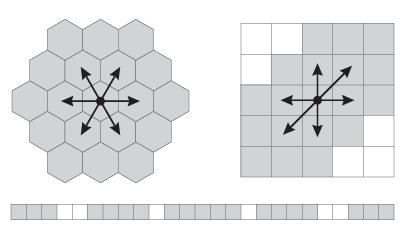
\includegraphics[width=0.7\textwidth]{pictures/Implementation/bitboards/hexa to cube.png}
    \caption{Translation from axial coordinate system to standard orthogonal system stored in a one dimensional array/bit \cite{browne2014bitboards}}
    \label{fig:hexa to cube}

    \hfill

  \end{subfigure}
  \begin{subfigure}{0.49\textwidth}
    \centering
    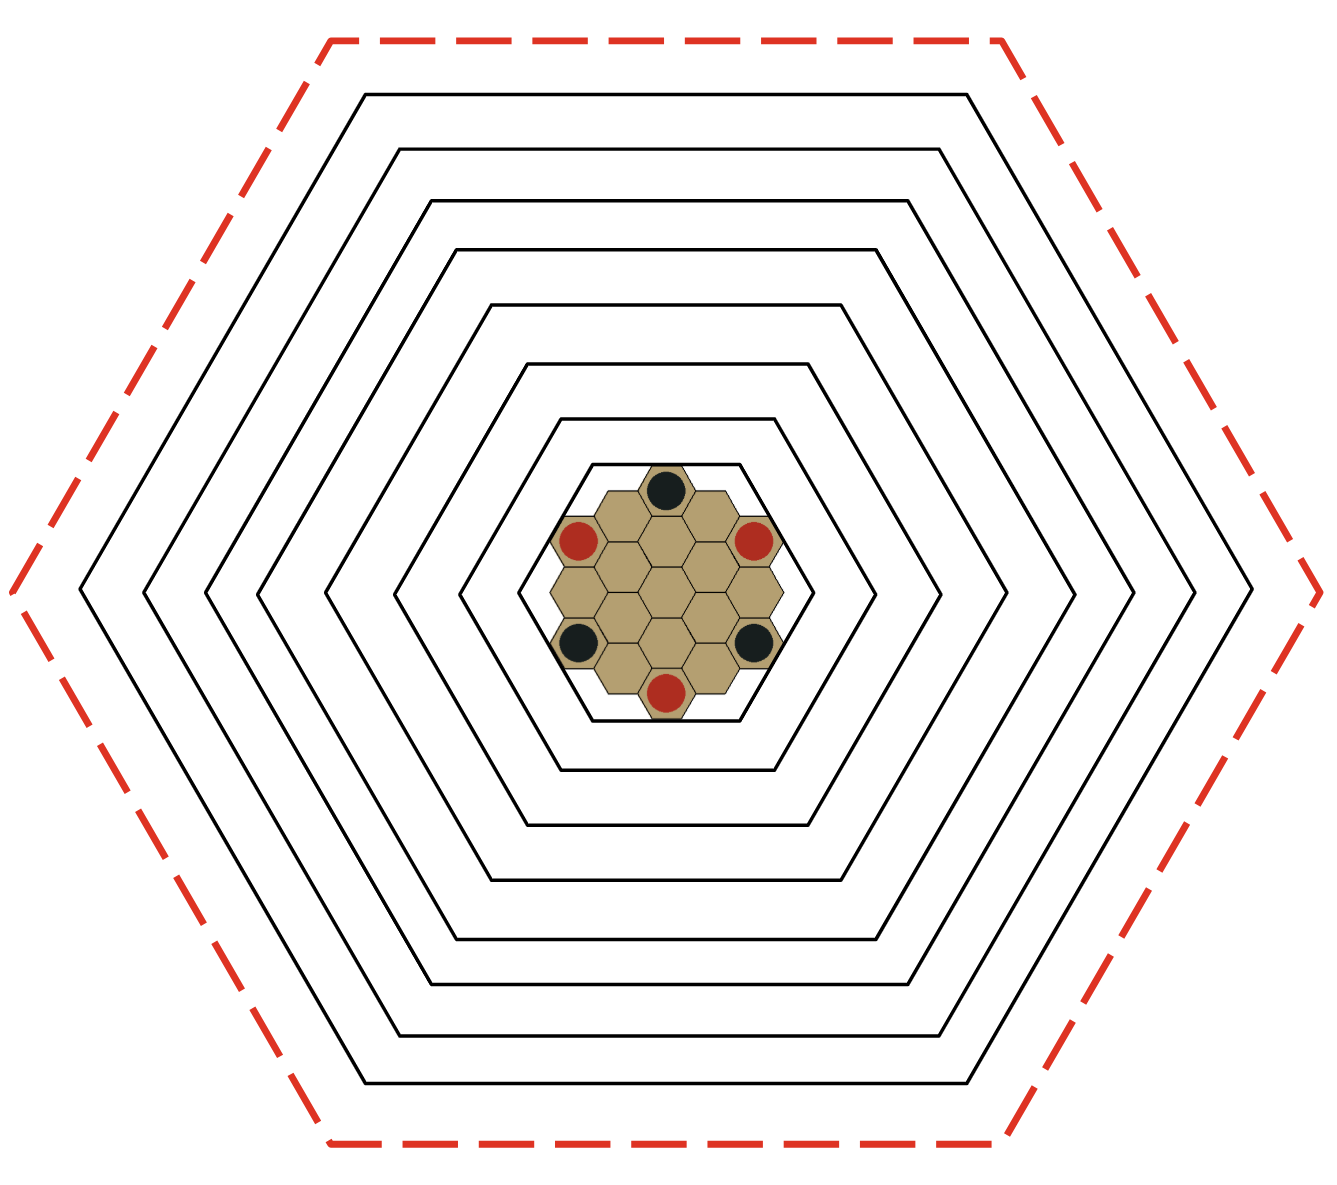
\includegraphics[width=\textwidth]{pictures/Implementation/bitboards/play-field.png}
    \caption{Play-field size visual representation}
    \label{fig:play-field}
  \end{subfigure}
  \caption{}
\end{figure}



To map the hexagonal board geometry into a linear bit sequence, the engine employs a coordinate transformation from an axial hex-coordinate system $(q, r)$ to a flattened one-dimensional index \cite{browne2014bitboards}. Because axial coordinates can be negative, a constant spatial offset (\texttt{BOARD\_OFFSET = 10}) is applied to shift the origin, ensuring all values fall within a non-negative range. The hexagonal space is subsequently embedded into a 2D square grid defined by \texttt{BOARD\_WIDTH = 10 + 1 + 10 = 21}. The linear index is then computed using row-major flattening:
$$ \text{index} = (q + 10) + (r + 10) \times 21 $$

This index directly targets a specific bit within the 448-bit span. To locate this bit in the array of seven 64-bit integers, the engine utilizes rapid bitwise operations: $\text{index} \gg 6$ (right shift by 6 to divide by $64=2^6$ ) yields the 64-bit word index, while $\text{index} \mathbin{\&} 63$ (bitwise AND with 63 equivalent to modulo 64) isolates the exact bit position within that word.\\

To illustrate this translation, consider a tile at the axial coordinate $q = -2, r = 0$. Applying the offset yields the non-negative coordinates $q_{\text{shifted}} = 8$ and $r_{\text{shifted}} = 10$. The row-major flattening then calculates a linear index of $8 + (10 \times 21) = 218$. Utilizing the bitwise operations, the engine determines the word index ($218 \gg 6 = 3$) and the bit position ($218 \mathbin{\&} 63 = 26$). Thus, the cell's state is stored precisely at the 26th bit of the 4th integer (index 3) in the bitboard array.\\

Conversely, to retrieve spatial geometry from a set bit, an inverse mapping is applied. The index is derived from the word and bit position: $$ \text{index} = (\text{word\_index} \times 64) + \text{bit\_position} $$
The $(q, r)$ axial coordinates are extracted via modulo operations ($\text{index} \bmod 21$) and integer division ($\lfloor \text{index} / 21 \rfloor$) respectively. This seamless bidirectional mapping strictly relies on primitive integer arithmetic, avoiding the overhead of complex data structures while accurately preserving hexagonal topology as illustrated in \cref{fig:hexa to cube}.\\



Because a single bit can only represent a binary state (e.g., ``occupied'' or ``empty''), the complete game environment cannot be modelled within a single flat array. Instead, the engine maintains distinct bitboards representing different logical layers of the game: red pieces, black pieces, all tiles, movable tiles, unmovable tiles, and a cache of valid tile destinations.

\begin{itemize}
  \item \textbf{red pieces:} an array of $7 \times 64$ bits in which a 1 corresponds to a red piece being present at the corresponding coordinate.
  \item \textbf{black pieces:} the same as red pieces but for black pieces.
  \item \textbf{all tiles:} an array of $7 \times 64$ where each 1 corresponds to a tile being present at the corresponding coordinate.
  \item \textbf{movable tiles:} a state representation where a bit value of 1 identifies a tile structurally free to be translated without violating Nonaga's rules.
  \item \textbf{unmovable tiles:} the disjoint complement to movable tiles under all tiles, tracking pieces that are currently pinned by surrounding geometry and blocked from movement.
  \item \textbf{valid tile destinations:} a continuously updated cache where set bits map to all legally permissible landing coordinates across the current board topology.
\end{itemize}

The primary advantage of this architecture is that game logic is no longer processed through costly memory allocations or nested loops over data structures. Instead, state evaluation is executed using hardware-sympathetic operations: flipping, testing, shifting, and scanning bits directly at the CPU level.


\subsection{Optimized Move Generation Algorithms}
To support the heavy computational demands of deep game tree searches (such as Alpha-Beta pruning), the engine's move generation must minimize CPU cycles. The engine achieves this through optimization layers, a few of which will be explained here.

\subsubsection{Bare Metal Legality Check}\label{O1 lookup}
Validating whether a single cell is a legal landing destination (\texttt{candidate\_is\_legal\_for\_tiles}) is the most frequently executed function in the engine. To optimize this, the engine avoids traditional spatial pathfinding entirely.

Legality of a tile move in Nonaga relies solely on the immediate topology of a cell (\cref{sec:tile_movement_legality}). Therefore, the engine only evaluates the six immediate neighbours of a candidate cell. The engine performs a mask to ask a binary question: ``Which neighbours are occupied?''

The answers for these six neighbours are packed into a single 6-bit integer (representing a value from 0 to 63). This integer is then used as a direct index into a precomputed 64-entry lookup table containing all legal local shapes. Because the complex geometric rules of the game are written into this lookup table at compilation, validating any candidate cell resolves in a few CPU instructions.

\subsubsection{Sparse Traversal and Global Caching}
While movable tiles possess distinct valid destinations (\cref{fig:possible moves 1,fig:possible moves 2}), there is typically a substantial intersection between their respective move sets.

\begin{figure}[H]\centering
  % --- First Figure ---
  \begin{minipage}{0.49\textwidth}
    \centering
    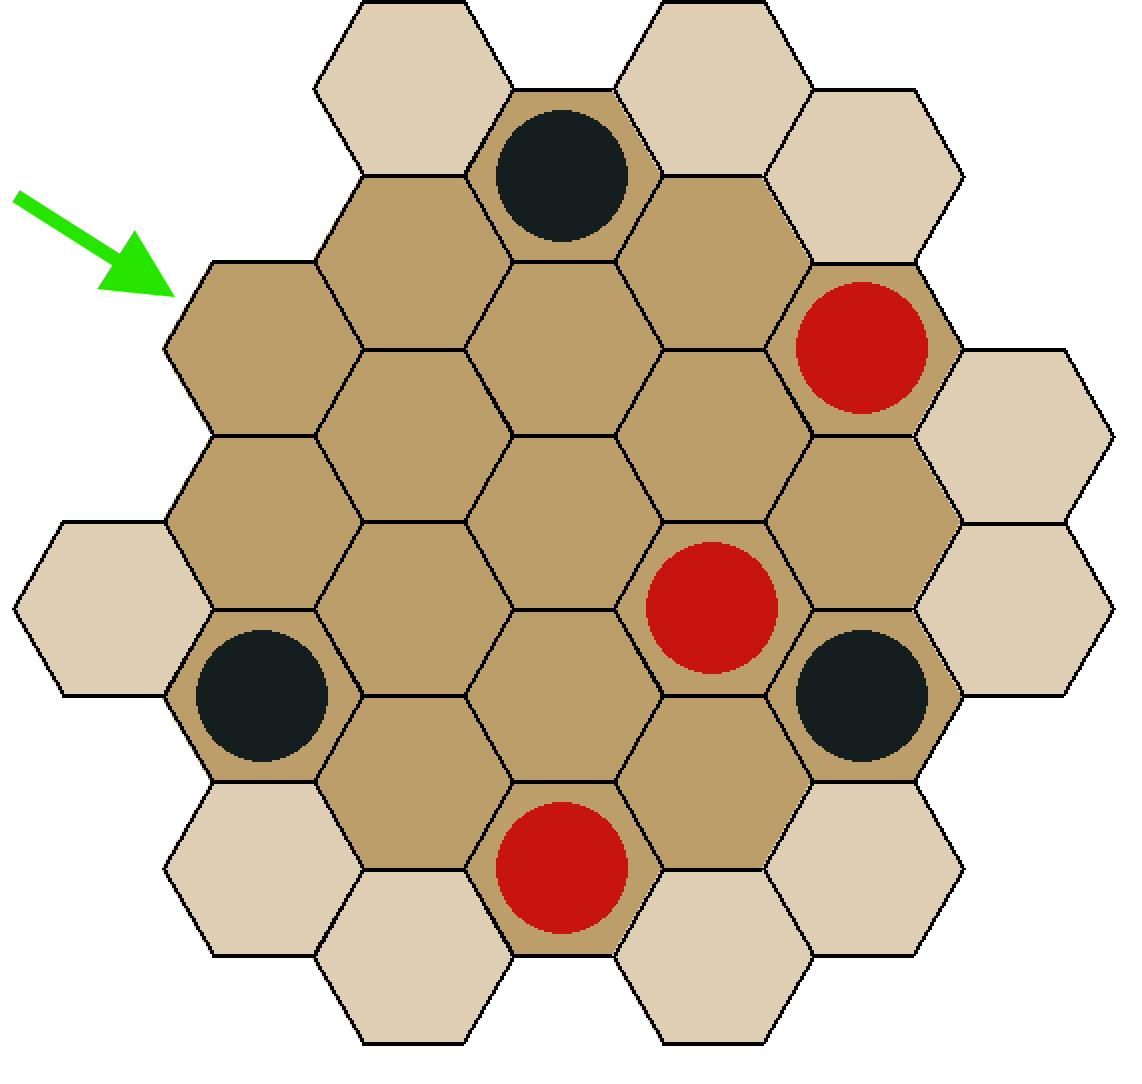
\includegraphics[width=0.5\textwidth]{pictures/Implementation/bitboards/possible destinations 1.png}
    \caption{The possible move set for the selected tile.}
    \label{fig:possible moves 1}
  \end{minipage}
  \hfill
  % --- Second Figure ---
  \begin{minipage}{0.49\textwidth}
    \centering
    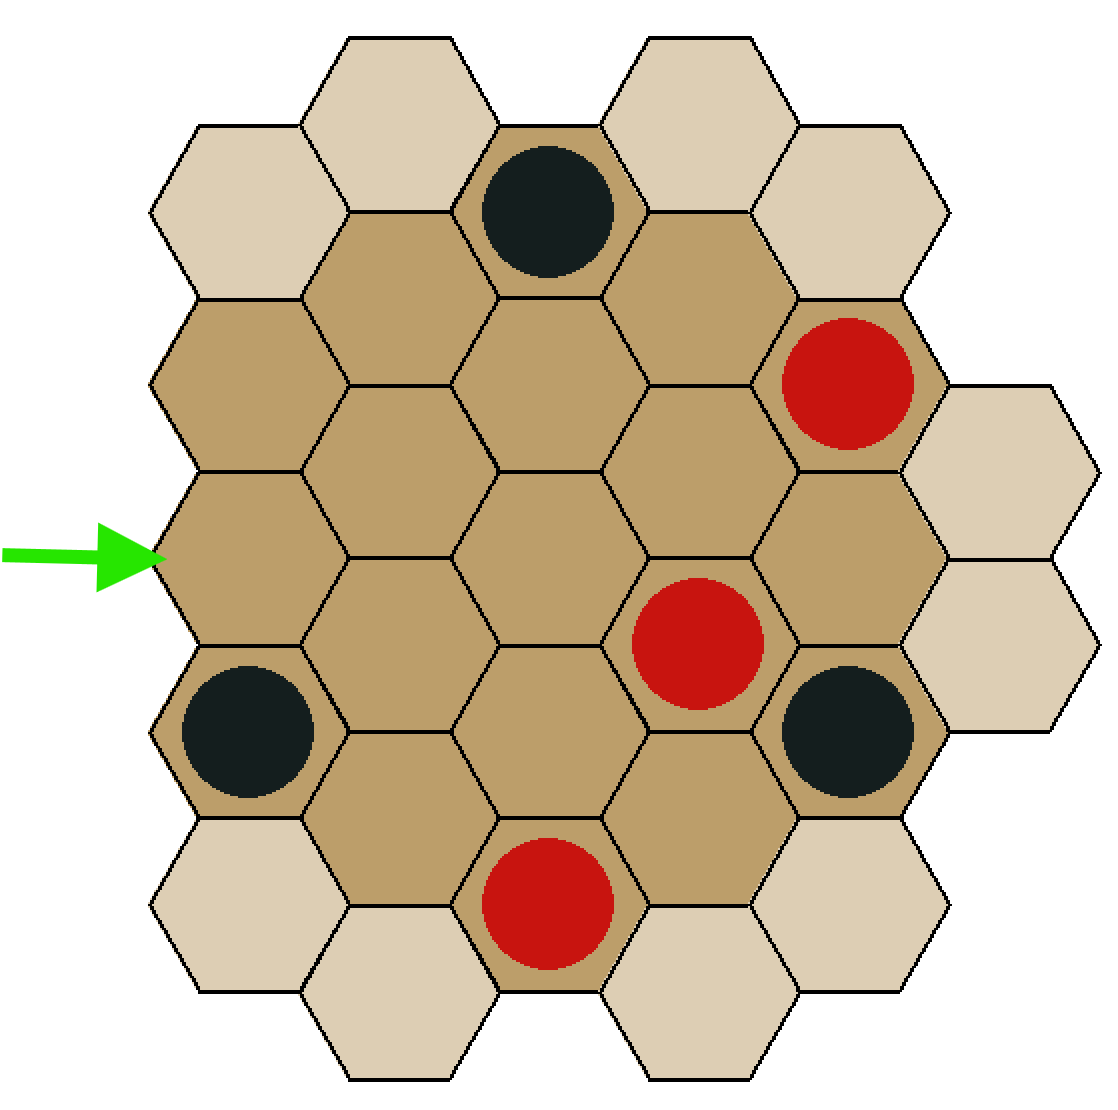
\includegraphics[width=0.5\textwidth]{pictures/Implementation/bitboards/possible destinations 2.png}
    \caption{The possible move set for an alternative selected tile.}
    \label{fig:possible moves 2}
  \end{minipage}
\end{figure}

To exploit this, the engine constructs a global cache of all theoretically legal destinations (\texttt{rebuild\_tile\_destination\_cache}). Rather than iterating through all 448 cells one-by-one, where the vast majority are empty space, the engine uses sparse bitboard traversal. By leveraging ``find next set bit'' hardware operations, the CPU jumps directly from one occupied tile to the next.

For each occupied tile found, its adjacent empty cells are recorded in a temporary bitset. Because multiple tiles might point to the same empty neighbour, writing this to a bitset inherently deduplicates overlapping cells. Only these specific, pre-filtered candidates are then passed through the bare metal legality check.

\subsubsection{Differential Move Generation}
When the engine needs to query the legal moves for one specific tile (\texttt{bitboard\_get\_valid\_tile\_positions\_for\_tile}), it employs a highly efficient differential update strategy.

Removing a source tile from the board logically alters the overall geometry. However, because legality is strictly dependent on immediate neighbours, removing a tile only affects the legality of its six immediate neighbours. Any cell farther away still possesses the exact same neighbour pattern as before.

The engine capitalizes on this mathematical guarantee by combining two methods. For any cell outside this 6-cell affected area, the engine completely trusts the global destination cache, instantly retrieving valid moves. The engine then distrusts the cache and re-runs the bare metal legality check only for the cells within the 6-cell subset. By utilizing the global cache for the majority of the board and only paying the computational cost for local rechecks near the moved tile, the engine achieves an exceptionally high work-per-instruction ratio.

\section{AI and Search Implementation}

\subsection{Zobrist Hashing for Transposition Table} \label{imp zobrist}

To optimize the Minimax search and handle the convergence of different move sequences into identical board states, a Transposition Table (TT) was implemented (\cref{back tt}). Because the Nonaga game state is compactly represented using a bitboard architecture (\cref{bitboard}), mapping it into a unique 64-bit ``fingerprint'' using Zobrist hashing is highly efficient. The process begins by initializing a table of pseudo-random 64-bit integers generated from a deterministic seed. Each potential feature of the game state (e.g., a red piece, black piece, or tile occupying a specific cell index) is assigned a unique random key. The global hash for a given position is then computed by applying the bitwise XOR operator to the keys of all present features. This approach is computationally efficient due to the order-independent property of XOR; the engine iterates through the bitboard’s seven 64-bit words, identifies set bits, and accumulates the corresponding keys without requiring expensive re-calculations.

\subsection{Transposition Table Integration and Best Move Ordering} \label{sec:tt_integration}
\subsubsection{Retrieval}
During evaluation, the recursive \texttt{ai\_minimax\_piece} and \texttt{ai\_minimax\_tile} routines probe the TT before enumerating and expanding candidate nodes. Upon a hit, the engine extracts the cached depth, evaluation score, bounding flags (\texttt{EXACT}, \texttt{LOWER}, \texttt{UPPER}), and historical best moves, rigorously validating them against the current board to prevent hash collision errors. If a valid entry meets the required search depth, it triggers an immediate cutoff: either returning exact evaluations directly, or tightening the search window ($\alpha \geq \beta$) using bound resolutions.

\subsubsection{Writing}
Upon completing a node, the engine writes its computed Zobrist hash, depth, heuristic value, bound flag, and best moves back into the indexed slot.

\subsubsection{Best Move Ordering}
This mechanism acts as the backbone for the AI's classical Iterative Deepening framework. Implemented as a fixed loop from depth 1 up to \texttt{max\_depth} (rather than a time-budgeted variant), each iteration resets the root state, runs a full minimax search, and overwrites the overall best move. This takes advantage of the TT and allows Best Move Ordering.

\subsection{Parameterized Evaluation Function}
The evaluation function utilizes a total of eight features and tuned weights to evaluate a position. Four weights are applied to features extracted from the current player's piece configuration, while the remaining four are applied to the opponent's configuration. The total heuristic value of a state $S$ is the difference between the player's features and the opponent's, formalized below.



\begin{figure}[H]
  \centering
  \begin{subfigure}{0.3\textwidth}
    \centering
    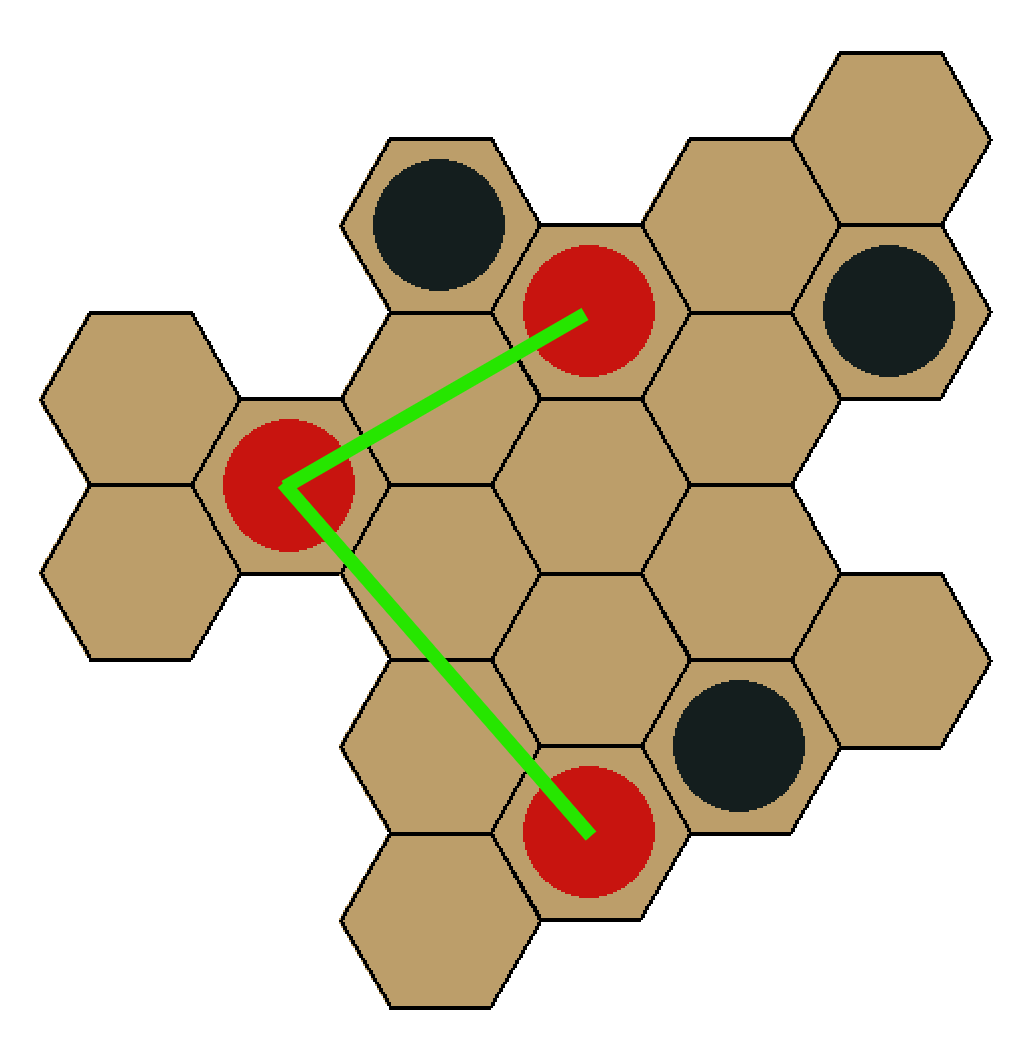
\includegraphics[width=\textwidth]{pictures/Evaluation Function/Euclidean Distance.png}
    \caption{Euclidean Distance}
    \label{subfig:feat1}
  \end{subfigure}\hfill
  \begin{subfigure}{0.3\textwidth}
    \centering
    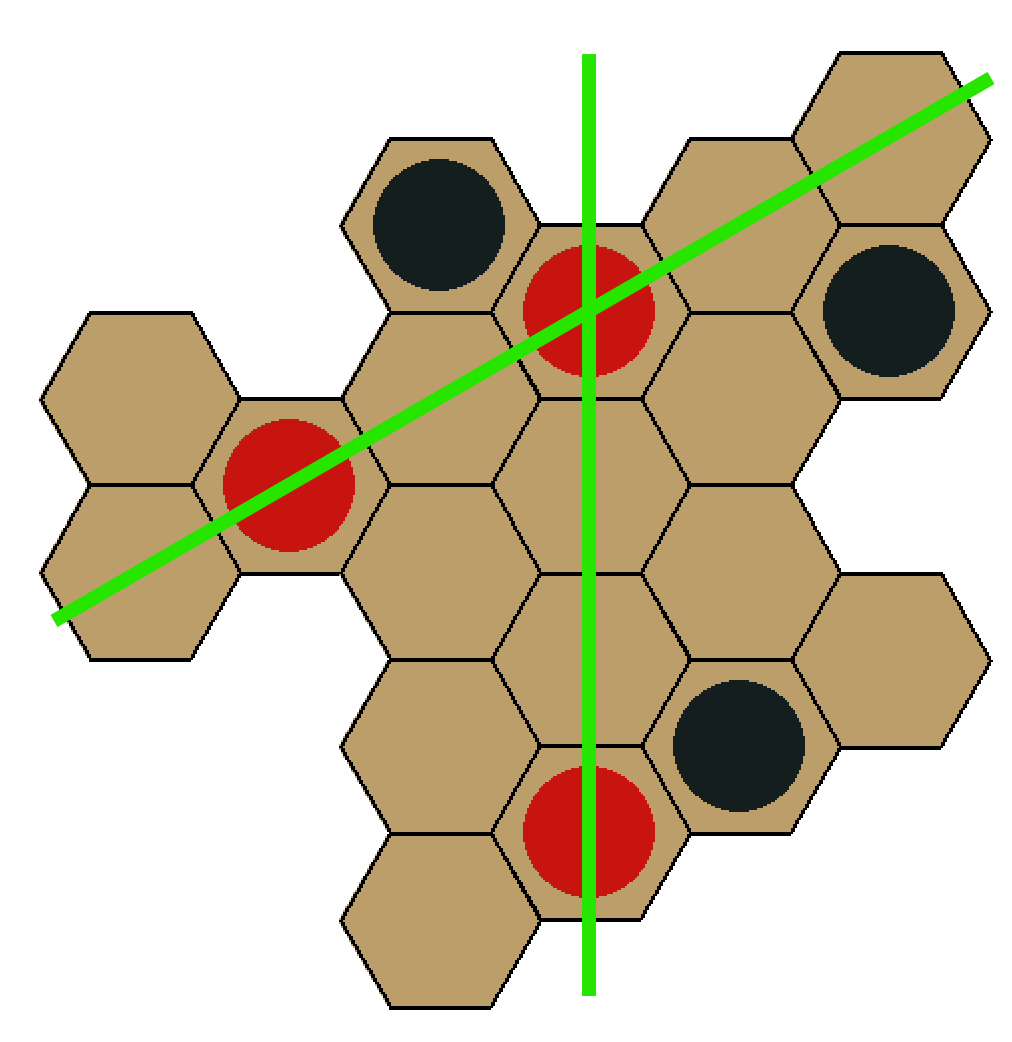
\includegraphics[width=\textwidth]{pictures/Evaluation Function/Alignement.png}
    \caption{Axis Alignment}
    \label{subfig:feat2}
  \end{subfigure}\hfill
  \begin{subfigure}{0.3\textwidth}
    \centering
    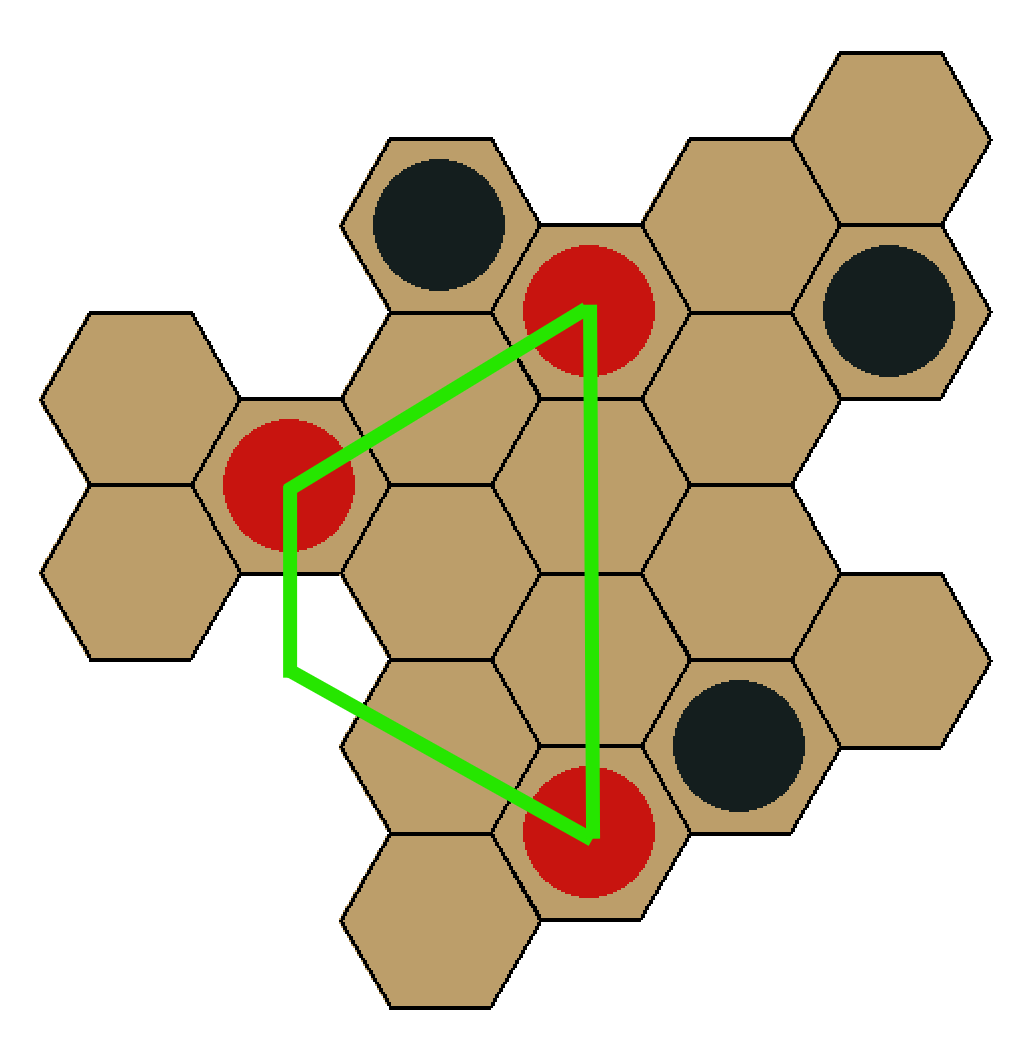
\includegraphics[width=\textwidth]{pictures/Evaluation Function/Tile and Enemies Area.png}
    \caption{Smallest bounding area containing the current player's pieces}
    \label{subfig:feat3}
  \end{subfigure}

  \caption{Visual support to the four heuristic features evaluated by the evaluation function.}
  \label{fig:eval_features}
\end{figure}


\begin{description}
  \item[1. Euclidean Distance:] As illustrated in \cref{subfig:feat1}, this feature quantifies the proximity of a player's pieces. Rather than calculating the total distance between all piece pairs, the heuristic sums only the two smallest distances. This approach accurately reflects the game's win condition: pieces only require a single adjacent neighbour to form a continuous chain. Minimizing these two specific distances directly facilitates the formation of a win-state without requiring redundant proximity between all three pieces.
  \item[2. Axis Alignment:]  This feature, visualized in \cref{subfig:feat2}, measures the degree to which a player's pieces share a common hexagonal axis. In the game’s mechanics, pieces move in straight lines until an obstacle is reached; therefore, aligning pieces on the same axis is a critical strategic precursor to forming a connection. The heuristic assigns a value ($0, 1, $ or $2$) based on the number of collinear pairs. Notably, even if all three pieces are mutually aligned on a single axis, the maximum value remains $2$, as this represents the minimum number of connections required to link three discrete points into a single continuous chain.
  \item[3. Missing Tiles:] This feature quantifies the ``missing'' space within the smallest bounding area containing a player's pieces (The area can be seen \cref{subfig:feat3}). In a dynamic hexagonal grid, empty spaces function as impassable voids that disrupt movement connection paths. A higher count of missing tiles increases the ``topological distance'' between pieces, forcing the agent to execute more complex, multi-turn manoeuvres to bridge the gaps. This forces the evaluation function to prioritize board configurations that maintain a solid, manoeuvrable surface.
  \item[4. Opponent Disruption:] Similarly to Feature 3, this feature counts the number of opponent pieces in the smallest bounding area containing a player's pieces (The area can be seen \cref{subfig:feat3}). A higher number of opponent pieces between the current player's pieces makes it easier for them to impede the current player's plans.
\end{description}



\section{The Genetic Algorithm Framework}
\label{sec:ga_framework}

\subsection{GA Architecture and Encoding}
The encoding strategy maps directly to the linear evaluation function, which requires eight distinct parameters. Consequently, a chromosome is represented as a continuous-like integer array of size eight, bounded within the interval $[0, 50]$. Each gene corresponds to a specific weight within the evaluation function.

\subsection{Fitness Evaluation via Tournaments}
To evaluate the fitness of each chromosome, a tournament-style selection process is employed. An AI agent equipped with a specific chromosome's weights competes against $k$ opponents drawn from the current population. The scoring system awards $1$ point for a win, $0$ points for a loss, and $0.5$ points for a draw. The cumulative score at the conclusion of the tournament serves as the chromosome's fitness value.

This approach is highly advantageous as it avoids making prior assumptions about opponent behaviour, thereby mitigating the risk of overfitting against a specific, static strategy. Because the pool of opponents dynamically evolves across generations, the evaluation metric is inherently robust. While there exists a theoretical risk of a single chromosome dominating the population and reducing genetic diversity, empirical observations during development indicated that this was not a prevalent issue.

\subsection{Selection, Crossover, and Mutation Operators}
Once fitness values are assigned, chromosomes are selected for reproduction using the Roulette Wheel Selection method \cite{Katoch2021}. The probability of a chromosome being selected is directly proportional to its fitness value divided by the aggregate fitness of the entire population.

For reproduction, the arithmetic crossover method is utilized \cite{Katoch2021}. Unlike combinatorial problems (such as the Travelling Salesman Problem) where genes represent distinct categorical nodes and arithmetic operations might yield invalid states, the genes in this context represent independent numerical weights. Therefore, arithmetic crossover does not risk violating structural constraints.

Finally, to maintain genetic diversity, a mutation function is applied. At each generation, every gene within the population possesses a predefined probability of mutation. If triggered, the gene is replaced by a uniformly distributed random integer within the $[0, 50]$ interval.






\section{Testing Approaches}

\subsection{Manual State Verification via Custom UI} \label{sec:freemove}
To rigorously validate the underlying game engine and the Minimax decision-making logic, a diagnostic testing harness was integrated directly into the graphical user interface. By engaging a 'Free Move' developer mode, the UI transitions from a standard game client into an interactive, visual debugging environment.

A critical feature of this harness is the ability to save and load arbitrary board states. This capability facilitated deterministic scenario testing, which is essential for isolating complex edge cases in adversarial search algorithms. For instance, specific board configurations where the opponent possessed an immediate, one-turn winning threat were manually constructed and injected into the engine. By triggering the AI's search function from these controlled states, it was possible to empirically verify whether the Minimax implementation correctly identified the sole ``loss evasion'' moves. This visual, scenario-driven approach proved invaluable for confirming the functional correctness of the heuristic evaluation function and the alpha-beta pruning logic without relying solely on opaque console outputs.

Furthermore, a chronological state traversal mechanism navigable via UI directional controls was implemented to audit the move history of a given session. During extended adversarial testing against the AI, this feature allowed for the step-by-step playback of the executed game tree. It served as a vital validation tool to ensure that the AI strictly adhered to the mathematical invariants of the game rules, guaranteeing that no illegal state transitions were generated or executed during deep, prolonged gameplay.

\subsection{Execution Time Profiling Methodology}

To mitigate the risk of performance degradation during the optimization phase, an empirical, profiling-driven methodology was adopted. Given the hybrid C/Python architecture of the project, performance bottlenecks were inherently difficult to isolate using standard Python profilers. Consequently, \texttt{py-spy} was utilized as a sampling profiler. To ensure complete visibility into the underlying C extensions during execution, the C codebase was compiled using \texttt{gcc} with debug symbols explicitly preserved (e.g., via the \texttt{-g} flag). Post-execution, the profiling data was exported to an SVG format to generate flame graphs. This visual representation of the call stack allowed for the immediate identification of heavily localized computational bottlenecks. Code optimization was then systematically managed through the following iterative lifecycle:

\begin{enumerate}
  \item \textbf{Bottleneck Identification:} Isolate the most computationally expensive function via flame graph analysis.
  \item \textbf{Targeted Optimization:} Refactor the algorithm to reduce temporal complexity or minimize invocation frequency (e.g., via bitboard manipulation enhancements).
  \item \textbf{Performance Verification:} Benchmark the targeted modification to confirm a statistically significant reduction in total execution time.
  \item \textbf{Regression Testing:} Ensure the optimization maintained strict functional correctness without introducing logical regressions.
\end{enumerate}

This continuous profiling loop was sustained until the Minimax algorithm achieved a stable execution time of a few seconds per move at a search depth of $d=3$. Scaling the search space to $d=4$ resulted in execution times exceeding 100 seconds per move. Because Minimax expands exponentially with respect to the branching factor ($O(b^d)$), further low-level optimization of the bitboard yielded diminishing returns. Therefore, a pragmatic architectural decision was made to terminate the optimization phase. A depth of 3 provided highly satisfactory AI proficiency, representing an optimal trade-off between computational tractability and heuristic search depth within the project's time constraints.

\subsection{Empirical Validation Of The Evolutionary Heuristic Optimization} \label{GA testing}

Early considerations of the GA's tournament selection highlighted a fundamental algorithmic challenge known as the ``relative fitness'' problem \cite{rosin1997new}. Because a candidate chromosome's fitness is evaluated by playing matches against a limited subset of the current population, its apparent viability is entirely dependent on its immediate neighbours. For instance, a globally excellent gene tested exclusively by other highly evolved genes might yield a mediocre win-rate and be incorrectly discarded. Conversely, an average gene situated in a poorly performing sub-population might appear exceptional, an issue that can ultimately lead to a loss of evolutionary gradient or co-evolutionary disengagement \cite{ficici2000game}.

To test the results of GA runs and to establish an objective performance baseline, supposedly elite chromosomes were systematically evaluated against a mostly fixed, heterogeneous benchmark pool rather than relying solely on intra-population play. This adversarial cohort was deliberately stratified into three categories:

\begin{itemize}
  \item \textbf{Stochastic Agents:} AI utilizing uniformly randomized weight vectors to establish an absolute minimum baseline of game-playing competence.
  \item \textbf{Legacy Iterations:} Chromosomes extracted from intermediate generations of the GA, serving as a control group to empirically track evolutionary progress over time.
  \item \textbf{Domain-Expert Agents:} Heuristic profiles constructed via manual parameter tuning (hand-crafted).
\end{itemize}

By aggregating the win/loss ratios across this diverse array of opponents, the tournament yielded a robust, objective fitness metric. This comprehensive scoring mechanism established a definitive performance hierarchy, successfully isolating the globally optimal chromosome and choosing which chromosome to use in the final version of the AI.




